\documentclass[8pt]{article}

\usepackage[T1]{fontenc}
\usepackage[utf8]{inputenc}
\usepackage{graphicx}
\usepackage{lmodern}
\usepackage{amsmath}
\usepackage{xfrac}
\usepackage{amsthm}
\usepackage{listings}
\usepackage{enumerate}
\usepackage{amssymb}
\usepackage{cancel}
\usepackage{amsfonts}
\usepackage{float}
\usepackage{fullpage}

\DeclareUnicodeCharacter{200A}{ } 
\renewcommand*\contentsname{Table des matières}

\PassOptionsToPackage{hyphens}{url}\usepackage{hyperref}

\usepackage{listings}
\author{ControverSciences\textit{ et al} }
\title{Projet AREN - Corpus de ressources \\ L’Arctique et ses enjeux géostratégiques}
\date{7 Mars 2018}

\begin{document}
\maketitle

\tableofcontents

\newpage
\section{Textes à débattre}

\subsection{ Arctique : comment exploiter et protéger ? }

\begin{itemize}
	\item \textbf{Lien : }  \url{http://www.ledauphine.com/politique/2014/07/10/arctique-comment-exploiter-et-proteger} 
	\item \textbf{Auteur : }  Aude Gambet, journaliste.
	\item \textbf{Date : } 11 juillet 2014
	\item \textbf{Source : } Le Dauphiné libéré est un journal quotidien de la presse écrite française régionale.
\end{itemize}

Dans le grand Nord, la fonte des glaces suscite la convoitise. Un rapport parlementaire s’interroge sur la façon d’exploiter les ressources de l’Arctique sans mettre en péril le système climatique et plaide pour une réelle politique.\\

Si les températures se réchauffent un peu partout sur la planète, le phénomène est encore plus important dans l’Arctique. Le Giec (Groupe d’experts intergouvernemental sur l’évolution du climat) envisage une hausse de l’ordre de 4 à 5 degrés d’ici à 2050 au-delà du cercle polaire contre 2 degrés sous nos latitudes tempérées. Parmi les conséquences de ce réchauffement, la banquise fond. Les terres du nord de l’Europe, de la Russie et du Canada se libèrent de leurs glaces, rendant plus accessibles d’importants gisements d’hydrocarbures.\\

Qui décide d’exploiter ces ressources ? « 95\% des ressources pétrolières de l’Arctique se situent dans la zone économique exclusive des États qui bordent l’océan », souligne le sénateur André Gattolin (Hauts-de-Seine, écologiste) dans un rapport rendu public hier. Chacun fait donc comme bon lui semble.\\

\textbf{Des grands groupes français déjà présents}\\

« L’Arctique est une partie du monde soumise à une gouvernance faible », poursuit le sénateur. Les pays riverains ont beau se réunir régulièrement dans le cadre du Conseil de l’Arctique, celui-ci « n’a pas le pouvoir d’édicter des normes » et reste « verrouillé » par ses membres. Trois États de l’Union européenne y siègent. Mais, privés d’accès à l’océan Arctique, deux d’entre eux, la Finlande et la Suède, sont considérés par les pays côtiers comme « des participants de second rang », observe André Gattolin.\\

Comment l’UE, et plus particulièrement la France, peuvent-elles avoir leur mot à dire sur cette région du globe stratégique d’un point de vue environnemental et économique ? Plusieurs grands groupes français (Total, GDF-Suez ou encore Areva) n’ont pas attendu d’avoir la réponse et travaillent déjà dans la région. Au sein de l’UE s’ébauche une politique commune en direction de l’Arctique : la Commission européenne doit soumettre ses propositions d’ici à la fin 2015. La France, présente en Arctique grâce aux scientifiques de l’institut Paul-Émile-Victor, doit de son côté se doter d’une feuille de route dans les mois qui viennent.

\newpage

\subsection{L’inquiétante course à l’Arctique}
\begin{itemize}
	\item \textbf{Lien : }  \url{https://www.lemonde.fr/idees/article/2015/08/07/l-inquietante-course-a-l-arctique_4715725_3232.html}
	\item \textbf{Date : } 7 août 2015
	\item \textbf{Source : } Le Monde
\end{itemize}

La Russie a de nouveau revendiqué mardi sa souveraineté sur 1,2 million de kilomètres carrés dans l’Arctique. Le Danemark et le Canada ont engagé une démarche similaire.\\

L’Arctique renfermerait 13\% des ressources mondiales de pétrole et 30\% de celles de gaz naturel, essentiellement en Russie et en Alaska ; même si les conditions climatiques extrêmes rendent encore leur exploitation très hypothétique et coûteuse, un tel pactole attise inévitablement les appétits. En outre, les compagnies maritimes voient dans la fonte rapide de la banquise ces dernières années une formidable occasion : entre la Chine et les marchés européen et américain, le trajet par le nord est bien plus court que celui passant par le canal de Suez.\\

Dans ce contexte, la Russie affiche toujours davantage son ambition de devenir la grande puissance polaire. Dès 2001, elle avait déposé à l’ONU, sans succès, une demande d’extension de sa « zone économique exclusive », très au-delà des 200 milles nautiques (370 kilomètres) qui sont la norme internationale. En 2007, à la stupeur générale, elle avait planté son drapeau en titane à 4 200 mètres de profondeur, sous le pôle Nord. Sur instruction du président Poutine, elle s’est, depuis, lancée dans une vaste militarisation de l’Arctique, ranimant notamment les anciennes bases soviétiques. Mardi 4 août enfin, sur la base des recherches géologiques et scientifiques menées ces dernières années, Moscou a de nouveau soumis aux Nations unies une requête revendiquant sa souveraineté sur 1,2 million de kilomètres carrés dans l’Arctique.\\

\textbf{Risque écologique}\\

Cette initiative russe n’est en rien une surprise. A l’exception des Etats-Unis, qui n’ont pas ratifié la convention de l’ONU sur le droit de la mer, tous les Etats riverains ont engagé la même démarche. La Norvège a obtenu dès 2009 l’extension de sa zone économique exclusive et négocié en 2010 un accord avec Moscou sur des zones litigieuses. Le Canada a déposé sa propre demande auprès de l’ONU en 2013 et le Danemark en 2014.\\


Il peut apparaître rassurant que les acteurs du grand jeu arctique empruntent, ainsi, la voie de la négociation internationale pour défendre leurs intérêts. Mais il est beaucoup plus inquiétant d’imaginer ce qui adviendra, demain, si leurs revendications sont satisfaites.\\

Car le risque écologique d’une exploitation des ressources de l’Arctique est immense. Fortement échaudés par la catastrophe de 2010 dans le golfe du Mexique, les ONG et les populations locales s’alarment ainsi, à juste titre, du danger de marées noires, qui seraient incontrôlables dans l’immensité arctique. Quant aux scientifiques, ils redoutent que la ruée sur le Grand Nord n’accélère le dérèglement de l’écosystème planétaire. Comme c’est le cas pour l’Antarctique, la gouvernance de l’Arctique mériterait un cadre plus collectif et plus soucieux de l’intérêt général. Hélas, on n’en prend pas le chemin.

\newpage

\section{Corpus de ressources}


\subsection{L’Arctique, bombe polaire }

\begin{itemize}
	\item \textbf{Lien : }  \url{http://www.lemonde.fr/cop21/visuel/2015/12/09/climat-cinq-cartes-pour-comprendre-les-enjeux-geopolitiques_4827788_4527432.html#/arctique} 
	\item \textbf{Auteur : }  Olivier Truc, correspondant au journal Le Monde pour les pays nordiques et baltes.	Infographie par Véronique Malécot et Henri-Olivier.
	\item \textbf{Date : } 13 décembre 2014
	\item \textbf{Source : } Le Monde
\end{itemize}

\textbf{Fonte catastrophique, rivalités politiques, appétits économiques… Ce fragile espace est sous pression.}\\

La fonte de la banquise continue à aiguiser les appétits en Arctique. A tel point qu’il a fallu la chute du prix du pétrole pour venir au secours des écologistes, très inquiets de la fragilité de la région. En septembre, la superficie de la banquise a atteint 4,63 millions de km², le quatrième chiffre le plus bas depuis le début des mesures satellites en 1979. Cette fonte de la glace de mer n’est pas seulement un problème pour les ours blancs et les chasseurs de phoque. Elle signifie la disparition de surfaces réfléchissantes qui renvoient la lumière solaire dans l’espace. Résultat, la planète absorbe plus de chaleur.\\

Les industriels et les commerçants, de leur côté, voient ces changements comme une aubaine, même si les obstacles sont nombreux. La seule route maritime actuellement pratiquée sur un plan commercial en Arctique est celle reliant l’Asie à l’Europe en passant par le nord de la Russie. Ouverte au transit international en 2009, entre fin juin et mi-novembre, la route du Nord-Est (RNE) a connu son pic de fréquentation en 2013, avec 71 navires, la plupart battant pavillon russe. Cela reste très modeste en regard du canal de Suez (17 148 bateaux en 2014) et n’est rentable qu’avec un prix modéré de location des brise-glace russes d’accompagnement et surtout un prix élevé du pétrole (au-delà de 50 dollars le baril). C’est à ces conditions que les vingt jours de traversée économisés par l’Arctique s’avèrent rentables par rapport à Suez. \\

Actuellement, le prix bas des carburants rend la RNE moins intéressante. En 2014, la quantité de marchandises en transit international a baissé à 300 000 tonnes contre 1,3 million en 2013 et la tendance s’accentue en 2015. La RNE est toutefois largement utilisée pour desservir les ports russes du Grand Nord, en particulier pour l’énorme projet gazier de Yamal. Ce trafic intérieur est passé de 2,8 millions de tonnes en 2013 à 4,5 millions de tonnes au 1er octobre 2015.\\

La baisse des prix du pétrole explique aussi en grande partie la prudence actuelle pour l’exploitation des ressources de l’Arctique. Un quart des ressources mondiales non découvertes de pétrole et de gaz se trouverait dans la région. Lancé une première fois il y a dix ans, ce chiffre avait donné la fièvre polaire à de nombreux industriels qui ont multiplié les projets. Après une décennie fébrile, la quête d’un nouvel eldorado s’avère décevante.\\

\begin{center}
	\makebox[\textwidth]{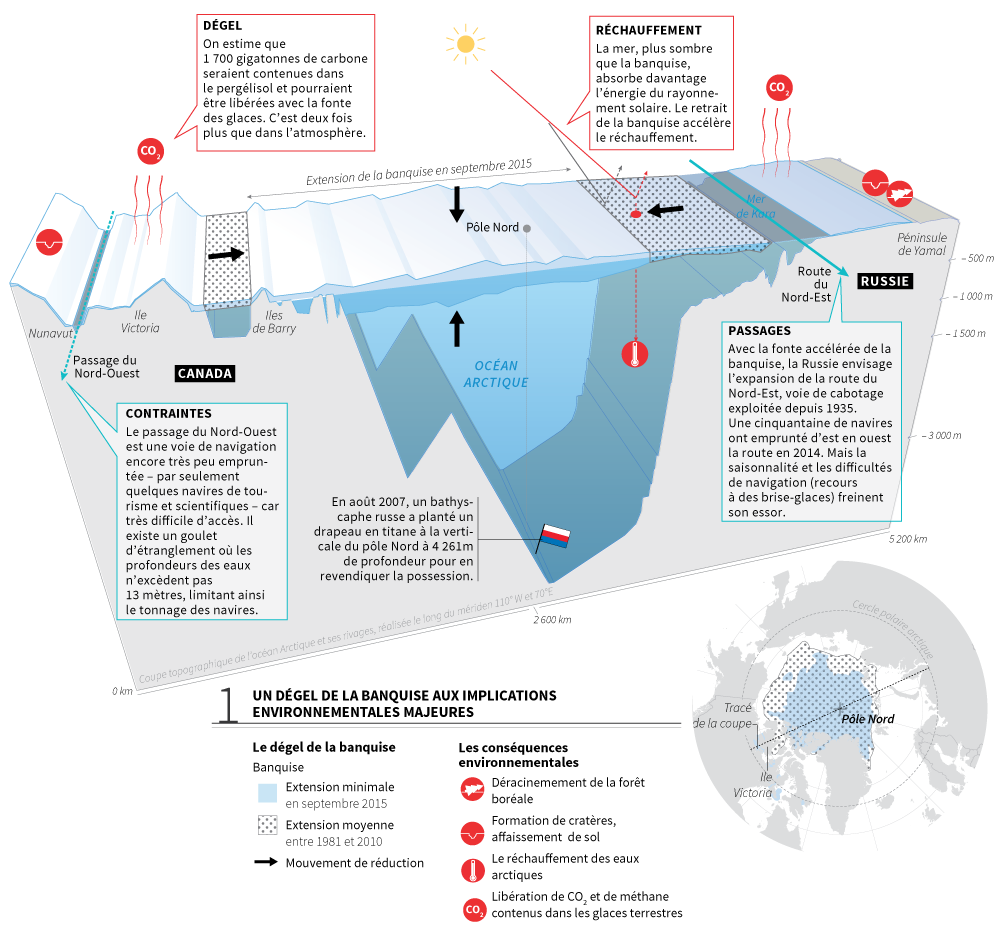
\includegraphics[width=\textwidth]{WEB-Arctique-partie1}}
\end{center}

Les Norvégiens de Statoil exploitent le gisement gazier de Snohvit au large du cap Nord depuis 2007 tandis que les Italiens d’ENI sont sur le point de démarrer l’exploitation du gisement pétrolier de Goliat, non loin de là. Côté russe, le premier gisement pétrolier dans l’Arctique est celui de Prirazlomnoye, dans le sud-est de la mer de Barents, en production depuis 2013. En mer de Beaufort, côté canadien, deux gros projets exploratoires, de Chevron et d’Imperial Oil, ont été suspendus cette année. Côté américain, Shell a annoncé fin septembre qu’il mettait fin à ses projets pétroliers peu concluants en mer des Tchouktches, au large de l’Alaska, et à la mi-octobre, le gouvernement américain a renoncé à vendre de nouvelles licences de forage dans l’Arctique.\\

Car outre les conditions économiques actuellement peu favorables, les obstacles à la ruée vers les terres polaires sont également techniques : compte tenu du climat hostile, avec des tempêtes fréquentes, travailler en Arctique, à de très grandes profondeurs, s’avère très ardu, et rien n’indique que les pétroliers sauraient faire face à une marée noire. D’autres menaces pèsent sur cette région, comme la surexploitation des ressources halieutiques, ainsi que les naufrages potentiels liés à la navigation en hausse.\\

Plusieurs organisations et personnalités ont plaidé en faveur de la sanctuarisation de l’Arctique, à l’instar de l’ancien premier ministre français Michel Rocard. Mais ce projet n’est pas soutenu par les puissances voisines qui ont toutes des velléités sur la zone. Elles se disent qu’à la différence de l’Antarctique, protégé par un traité international, l’Arctique est habité par plusieurs millions de personnes qui ont besoin de perspectives de développement.

\begin{center}
	\makebox[\textwidth]{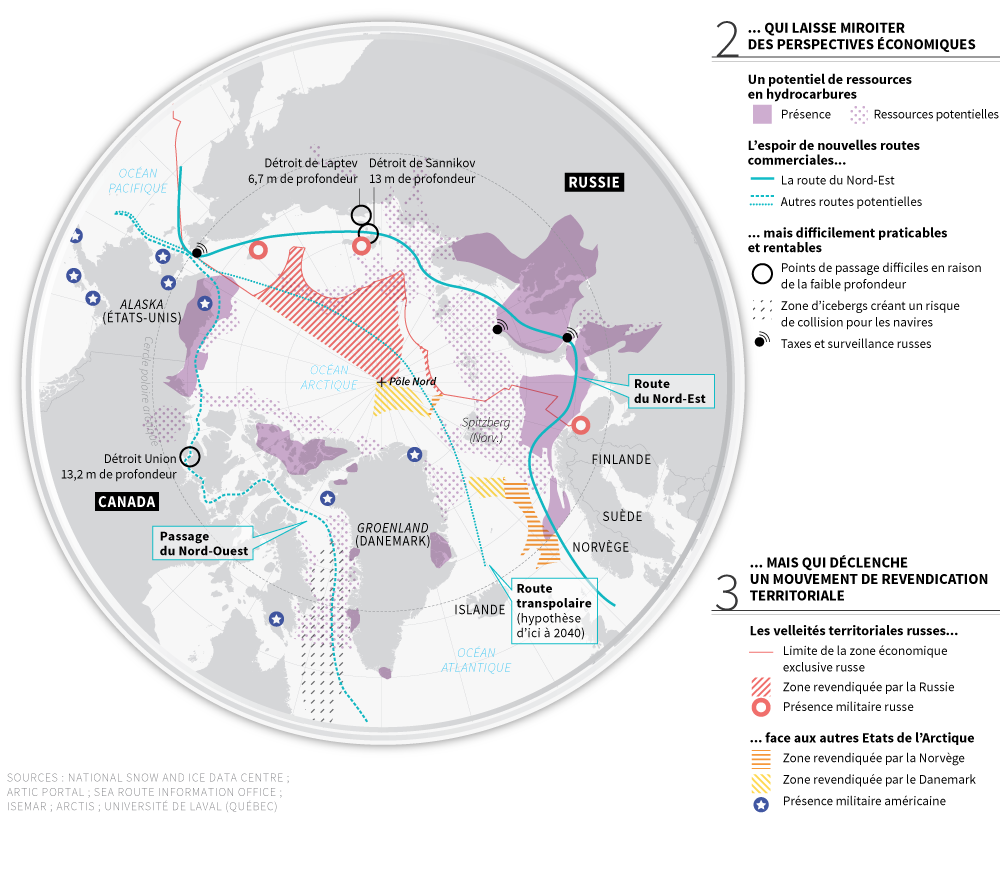
\includegraphics[width=\textwidth]{WEB-Arctique-partie2-3}}
\end{center}

\newpage

\subsection{Arctique, la fin du sanctuaire - Le dessous des cartes}

\begin{itemize}
	\item \textbf{Lien : }  \url{http://ddc.arte.tv/nos-cartes/arctique-la-fin-du-sanctuaire} 
	\item \textbf{Auteur : }  Jean-Christophe Victor, ethnologue et fondateur du Laboratoire d’études politiques et d’analyses cartographiques.
	\item \textbf{Date : } 13 décembre 2014
	\item \textbf{Description : } L’Arctique était le bout du monde. Le réchauffement climatique va-t-il le placer au centre des préoccupations géopolitiques ? Pétrole, gaz, terres rares, les convoitises sont nombreuses. Quelles menaces cela fait-il peser sur le monde polaire ? Le Dessous des Cartes s’intéresse à cette région située aux marges du planisphère.
	\item \textbf{Source : } Le Dessous des cartes est une émission éducative hebdomadaire, elle a pour but de traiter un sujet de géopolitique et de géographie principalement par le biais de cartes géographiques.
\end{itemize}

\subsection{Arctique : le changement climatique redessine les relations internationales}

\begin{itemize}
	\item \textbf{Lien : }  \url{http://arctique.blog.lemonde.fr/2016/04/28/arctique-le-changement-climatique-redessine-les-relations-internationales/} 
	\item \textbf{Auteur : }  Damien Degeorges, géopolitologue. Docteur en sciences politiques, après une thèse de relations internationales consacrée au rôle du Groenland dans les enjeux de l’Arctique, diplômé en communication politique et en études nordiques. Il coordonne, en tant que chercheur associé, l’initiative Norden, plateforme d’échanges franco-nordiques de l’Institut français des relations internationales.
	\item \textbf{Date : } 28 avril 2016
	\item \textbf{Source : } Planète Arctique, Enjeux stratégiques d'une région monde.
\end{itemize}

Comment une région peut-elle passer du statut de périphérie à celui de nouvelle frontière des relations internationales en moins d’une décennie ? C’est, dans le cas de l’Arctique, une conséquence directe du changement climatique. De cette région, où la hausse des températures est bien supérieure à la moyenne mondiale, dépend une partie importante de l’avenir de la planète, tant par la hausse du niveau des mers et des océans consécutive notamment à la fonte de la calotte glaciaire du Groenland que par la libération du méthane présent dans l’Arctique, pour ne citer que quelques exemples. L’attention portée aux nouveaux enjeux économiques et géopolitiques de l’Arctique remonte symboliquement au 3 août 2007, lorsqu’un drapeau russe avait été déposé à la verticale du pôle Nord. Depuis, l’intérêt international pour cette région n’a cessé de croître.\\

L’Arctique est actuellement le cas d’école par excellence des conséquences du changement climatique sur les relations internationales. La région n’est pas une nouvelle venue sur la scène internationale, comme l’a notamment démontré la Guerre froide, mais son exposition internationale est sans précédent. Comme en témoigne la popularité du statut d’observateur permanent au Conseil de l’Arctique, forum intergouvernemental crée en 1996, dont les Etats-Unis assurent actuellement la présidence tournante. La présence au sein de ce Conseil, à différents niveaux, de l’ensemble des acteurs du G7/G8 et de puissances comme la Chine et l’Inde offre à ce mini G20 une visibilité mondiale rare pour un forum régional. Outre les cinq pays nordiques (le Danemark via le Groenland, la Finlande, l’Islande, la Norvège et la Suède), l’Arctique comprend le Canada, les Etats-Unis et la Russie, qui de par notamment sa superficie arctique fait figure de puissance régionale.\\


L’Arctique n’est pas seulement un thermomètre du changement climatique. Les tensions géopolitiques s’observent également dans ces latitudes, notamment lorsque les relations se tendent entre la Russie et les pays de l’Organisation du traité de l’Atlantique Nord (OTAN). Les rapports de force à l’échelle mondiale ne sont cependant pas toujours les mêmes à l’échelon régional, comme cela se vérifie dans le Grand Nord. De par sa singularité, l’Arctique offre une autre lecture du monde, notamment grâce à une diplomatie climatique et scientifique qui permet à de grandes puissances, souvent rivales, de briser la glace. Ou quand Chine, Etats-Unis, Inde, Russie et d’autres se retrouvent loin des salles de réunion habituelles.\\

\textbf{De nouvelles opportunités dans un environnement fragile}\\

Le changement climatique a ouvert de nouvelles opportunités économiques dans l’Arctique. L’accès aux ressources naturelles (les hydrocarbures, de nombreux minerais parmi lesquels les stratégiques terres rares, des ressources halieutiques migrant vers le Nord du fait du réchauffement des mers et des océans, ainsi que l’eau douce, stratégique sur le long terme, dont environ 10\% des réserves mondiales se trouvent au Groenland) et le développement des routes maritimes arctiques (le nombre de transits est à ce jour limité, en comparaison aux routes maritimes traditionnelles du commerce international, mais la route empruntant le passage du Nord-Est et longeant la Russie s’apparente à un accélérateur de la mondialisation, de par la réduction considérable des distances entre Asie et Europe qu’elle engendre) s’en trouvent facilités.\\

Une fois le constat établi, force est de constater que l’environnement de la région est fragile et que les conditions peuvent être extrêmes. De par ses caractéristiques, l’Arctique a la possibilité de devenir le modèle d’un développement économique durable.\\

Sur le plan de la configuration, l’Arctique n’est pas l’Antarctique : peuplée d’environ 4 millions d’habitants, la région entourant le pôle Nord est un océan bordé d’Etats souverains, libres de décider du développement de leur zone arctique. Seul un espace autour du pôle Nord, en cours de délimitation du fait de demandes d’extension des limites du plateau continental de certains pays riverains de l’océan Arctique, n’appartient à personne.\\

Une prise de conscience au sein des entreprises participant au développement de l’Arctique est en train de s’opérer, car à l’évidence, au-delà du risque environnemental, le risque d’image et de notoriété en cas d’accident dans un environnement qui, dans l’inconscient général, reste synonyme de pureté, est trop grand pour toute entreprise qui se respecte.\\

\textbf{Une importance stratégique mise en évidence par la Chine}\\

Sur le plan de la géopolitique et de la recherche sur le climat, les deux pôles se rejoignent cependant. La pénétration d’une puissance comme la Chine dans ces régions polaires, par le biais notamment de la recherche, occuperait sans doute, à elle seule, tout un blog. L’Arctique doit en grande partie à la Chine l’exposition internationale qui est la sienne depuis plusieurs années. Aujourd’hui, les développements de la région arctique sont suivis jusqu’en Océanie.\\

L’Arctique, seule région à lier les grands blocs de l’économie mondiale que sont actuellement l’Amérique, l’Europe et l’Asie, est un véritable laboratoire des enjeux du XXIème siècle : changement climatique, sécurité énergétique, coopération entre puissances rivales, commerce international, notion d’indépendance, etc.\\

Regarder le monde d’en haut conduit à l’observer sous un angle différent, ce qui permet parfois de mieux comprendre certains enjeux mondiaux. La région-monde Arctique, c’est sûr, ne perd pas le Nord.
\end{document}


